\scanpage{14}
\figure{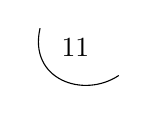
\begin{tikzpicture}[x=1cm,y=1cm]
\node at (0,0) {\mspage{11}};
\draw (-.45,.25) .. controls (-.6,-.4) and (.1,-.65) .. (.55,-.35);
\end{tikzpicture}}
\[
\left\{\begin{aligned}
L\Lambda&=1-\sum_{0\leq i\leq n}\pi_{i,0}\\
\Lambda L&=1-\sum_{n\leq j\leq2n}\pi_{\deleted{\unsure{2}}j,0}
\end{aligned}\right.
\tag{6.15}
\]
\deleted{Quant aux $\pi_{j,0}$, ils sont déterminés par les}

\uline{Question} Donner un système de \deleted{\unsure{générateurs}} relations entre les $\Lambda,L$ exclusivement, \deleted{\unsure{et}} \unsure{de|des} relations exprimant les $\pi_i$ comme polynômes en $L,\Lambda$ .... --- qui définissent $\Lambda$ en termes de $L$ et des $\pi_i$ ....
\margin{\figure{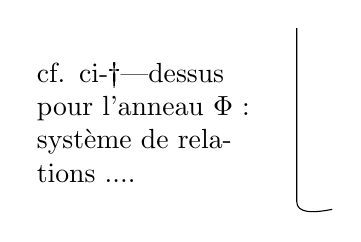
\begin{tikzpicture}[x=1cm,y=1cm]
\node[align=left,text width=3cm] at (0,0) {cf. ci-\unsure{†|dessus}\\pour l'anneau $\Phi$ :\\système de relations ....};
\draw (1.8,1.2) -- (1.8,-1) .. controls (1.8,-1.15) and (2,-1.15) .. (2.25,-1.1);
\end{tikzpicture}}}

7. Revenant à un anneau gradué abstrait $\mathcal E$, muni d'un
\[
L\in\mathcal E^{(2)},
\]
on veut abstraire la situation qui précède, sans utiliser $M^*$, en termes des propriétés du seul anneau \deleted{$\unsure{\mathcal E}$} gradué $\mathcal E^*$ muni de $L\in\mathcal E^{(2)}$.
Partons pour ceci \deleted{de} d'un module libre $\mathbf M_0$ de rang $2n$ sur $\mathbb Z$, muni d'une $2$-forme alternée non dégénérée \inserted{\figure{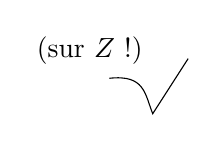
\begin{tikzpicture}[x=1cm,y=1cm]
\node at (0,.25) {(sur $\mathbb Z$ !)};
\draw (.25,-.1) .. controls (.7,-.05) and (.7,-.3) .. (.8,-.55) -- (1.25,.15);
\end{tikzpicture}}} $\xi_0\in\bigwedge^2\mathbf M_0$, \inserted{\figure{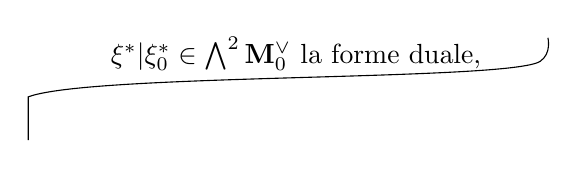
\begin{tikzpicture}[x=1cm,y=1cm]
\node at (0,.3) {$\unsure{\xi^*|\xi_0^*}\in\bigwedge^2\mathbf M_0^\vee$ la forme duale,};
\draw (-3.4,-.8) -- (-3.4,-.25) .. controls (-2.6,.05) and (2.7,-.05) .. (3.1,.2) .. controls (3.25,.3) and (3.2,.5) .. (3.2,.5);
\end{tikzpicture}}} soit \deleted{$\unsure{\xi}$} $\mathbf M_0^*=\bigwedge\mathbf M_0$, et considérons sur $\mathbf M_0^*$ les opérateurs
\[
\unsure{\mathbf L|\mathbf L_0}x=\xi_0x,\qquad\boldsymbol\Lambda_0x=\xi_0^*\mathbin{\lrcorner}x
\]
et considérons l'algèbre
\[
\Phi_0=\mathbb Z[\mathbf L_0,\boldsymbol\Lambda_0]\subset\operatorname{End}_{\mathbb Z}(\mathbf M_0^*)
\]
\margin{anneau gradué.}
Notons que $\operatorname{End}(\mathbf M_0^*)$, \inserted{\figure{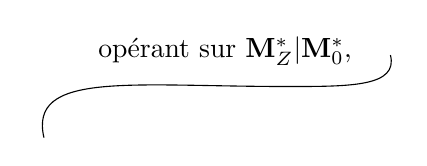
\begin{tikzpicture}[x=1cm,y=1cm]
\node at (0,.35) {opérant sur $\unsure{\mathbf M_{\mathbb Z}^*|\mathbf M_0^*}$,};
\draw (-2.3,-.75) .. controls (-2.5,.1) and (-1.2,-.1) .. (.8,-.1) .. controls (1.6,-.1) and (2.2,-.1) .. (2.1,.3);
\end{tikzpicture}}} muni de $\unsure{\mathbf L|\mathbf L_0}$, satisfait à la condition de $(6.1)\unsure{(i)|_i}$, \deleted{\unsure{donc}} et \deleted{$\unsure{\xi}$} $\boldsymbol\Lambda_0$ est l'opérateur associé défini par $(6.5)$.
\mspage{13}
